\chapter{State of the Art in Optimal V2G Management}

\section{The V2G Imperative: A Foundation of Europe's Green Transition}

Europe finds itself at the confluence of two unprecedented transformations: the wholesale electrification of transport and a fundamental restructuring of energy systems. These are not merely aspirational goals but constitute binding legal obligations enshrined in the \textbf{European Green Deal} and its comprehensive \textbf{"Fit for 55"} legislative framework \footcite{european_commission_2021_fit_for_55}. The policy architecture demands a 55\% reduction in net greenhouse gas emissions by 2030, necessitating the rapid elimination of internal combustion engines alongside a dramatic expansion of renewable energy capacity, as outlined in the revised \textbf{Renewable Energy Directive }(RED III). Electric Vehicles (EVs) occupy a central position in this transition, simultaneously driving decarbonisation efforts while presenting complex challenges for grid stability and management.
\noindent

\begin{figure}[H]
    \centering
    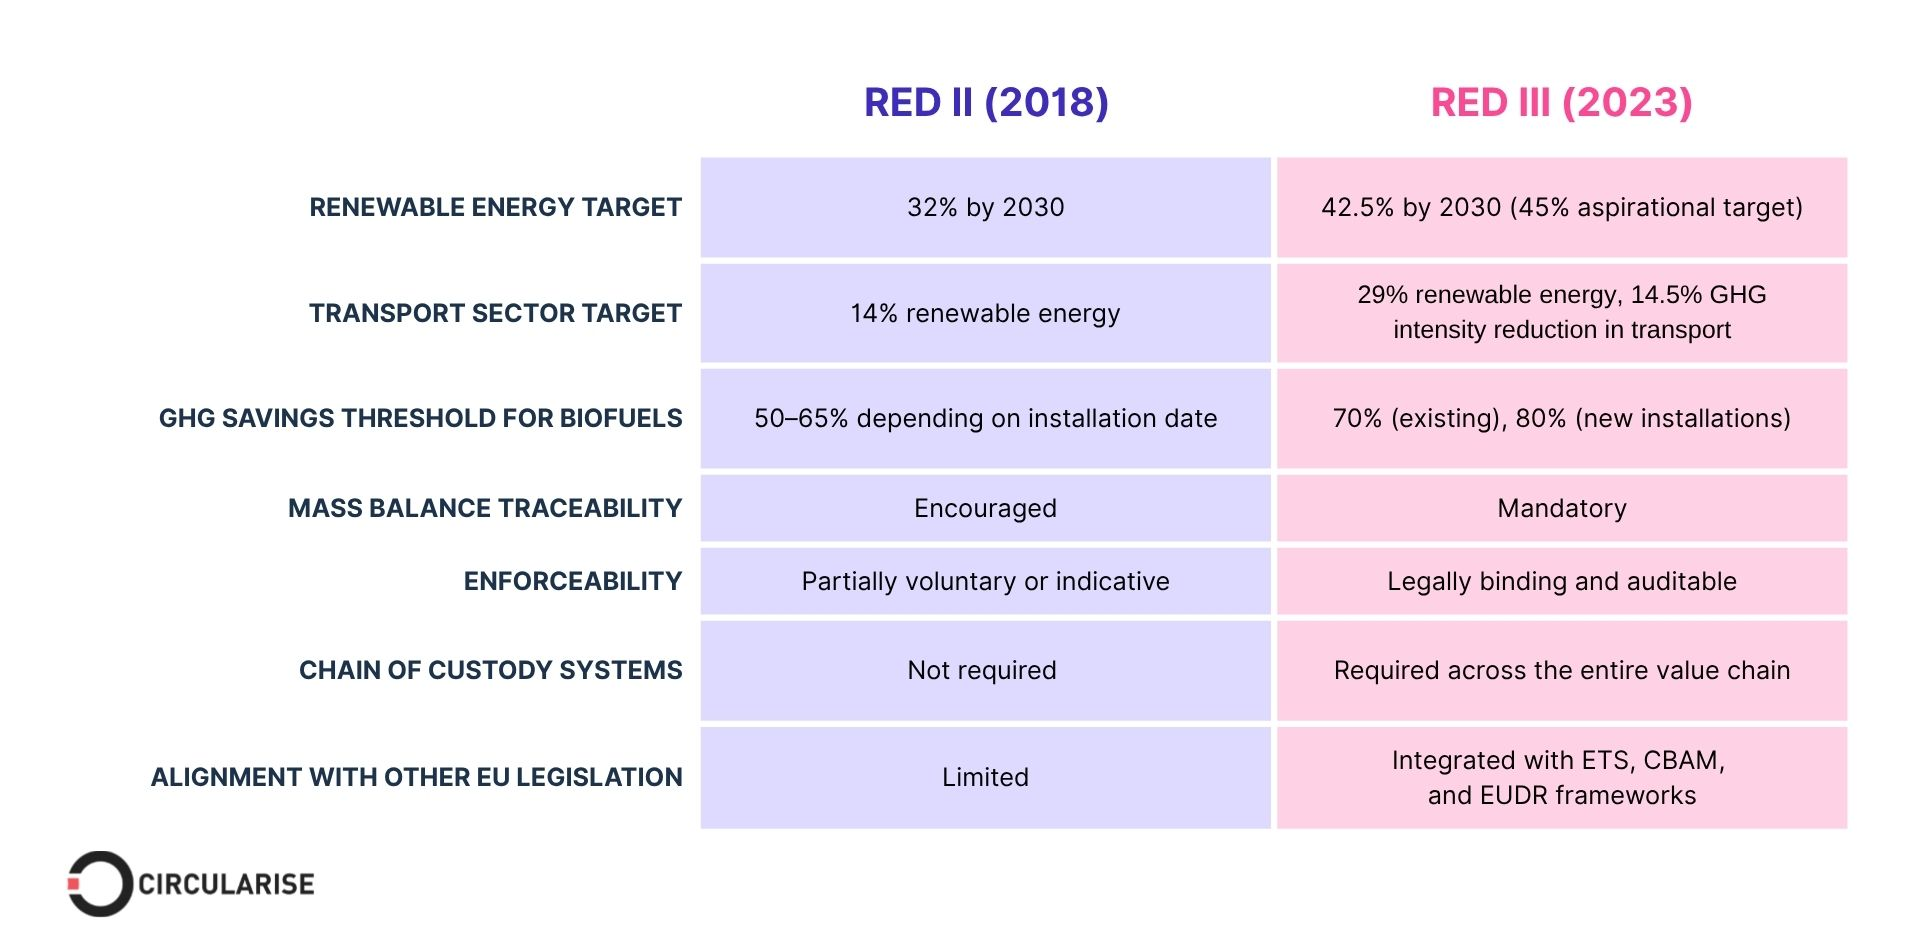
\includegraphics[width=0.75\linewidth]{red.jpg}
    \caption{RED 3}
    \label{fig:placeholder}
\end{figure}
\noindent
The initial response to mass EV adoption was characterised by considerable concern within the power sector. The prospect of millions of new electric vehicles was perceived primarily through the lens of risk—vast, temporally correlated loads threatening to overwhelm local distribution networks during peak evening hours. This perspective has undergone a fundamental reassessment. EVs are now recognised not as burdens to be managed, but as essential infrastructure for achieving Europe's energy transition objectives. This conceptual shift finds its most concrete expression in \textbf{Vehicle-to-Grid (V2G)} technology, which fundamentally reimagines the role of electric vehicles within the energy system.
\noindent
V2G technology transforms what were previously passive, unidirectional energy consumers into active, distributed, and smart grid resources. The underlying opportunity is both elegant and substantial: private vehicles spend approximately 96\% of their operational lifetime parked and connected \footcite{evertsson2024investigating}, representing an enormous, geographically distributed, and currently underutilised repository of mobile energy storage capacity.
\noindent
The transformative potential of V2G becomes apparent when individual vehicles are coordinated through centrally managed aggregation. While a single EV's contribution remains modest, a carefully orchestrated fleet can function as a unified entity—a \textbf{Virtual Power Plant (VPP)}. These software-defined power plants aggregate the collective capacity of numerous distributed energy resources, delivering grid services at scales and reliability levels comparable to conventional generation facilities. The rapid response characteristics of contemporary battery inverters, operating at millisecond timescales, enable these aggregated fleets to provide a comprehensive range of critical grid services. This capability extends beyond mere utility; it represents a prerequisite for maintaining stability in grids increasingly dependent on the variable and non-dispatchable output of wind and solar generation, thereby enabling the technical and economic viability of the EU's ambitious renewable energy targets \footcite{Tavakoli2019}.
\noindent
The grid services enabled by V2G technology form the technical foundation for the smart, resilient, and decarbonised electricity system required for Europe's energy future:

\begin{itemize}
    \item \textbf{Frequency Regulation:} Grid stability fundamentally depends on maintaining precise equilibrium between electricity supply and demand, manifested as stable grid frequency (50 Hz across European networks). Frequency deviations signal supply-demand imbalances that, if uncorrected, can trigger cascading failures across interconnected systems. V2G fleets, leveraging their rapid response capabilities, can participate directly in ancillary service markets including Frequency Containment Reserve (FCR) and automatic Frequency Restoration Reserve (aFRR). These systems can inject or absorb power within seconds of frequency deviations, providing immediate counteraction to imbalances and preventing system-wide failures or blackouts \footcite{alfaverh2022optima, white2011vehicle}.
    
    \item \textbf{Demand Response and Peak Shaving:} Through intelligent temporal shifting of charging activities to off-peak periods—when energy is abundant and inexpensive—combined with strategic discharging during peak demand when energy becomes scarce and costly, V2G systems can effectively flatten daily load profiles. This approach directly addresses the "duck curve" phenomenon associated with high solar photovoltaic penetration. Such load profile management reduces dependence on expensive and carbon-intensive "peaker" plants, typically gas or diesel turbine facilities, while potentially deferring or eliminating requirements for costly transmission and distribution infrastructure upgrades \footcite{orfanoudakis2022deep, sadeghi2021deep}.
    \begin{figure}[H]
        \centering
        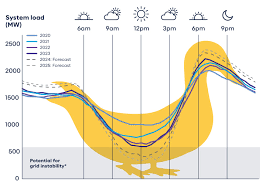
\includegraphics[width=0.75\linewidth]{duck.png}
        \caption{Duck curve}
        \label{fig:placeholder}
    \end{figure}
    
    \item \textbf{Renewable Energy Integration:} The most strategically significant contribution of V2G lies in addressing renewable energy intermittency challenges. V2G fleets function as large-scale energy buffers, absorbing excess solar and wind generation during periods of high production and low demand that would otherwise require curtailment. This stored renewable energy can subsequently be released during periods of low generation, such as evening hours or periods of limited wind availability. This mechanism directly increases the utilisation efficiency of renewable energy resources, supporting the integration objectives outlined in RED III while enhancing overall energy system efficiency \footcite{khan2024review, zou2021deep}.
\end{itemize}
\noindent
This vision is being actively incorporated into European legal frameworks and technical standards. The transformative \textbf{Alternative Fuels Infrastructure Regulation (AFIR, EU 2023/1804)} now requires that new public charging infrastructure incorporate smart charging capabilities and, critically, bidirectional power flow capacity. The technical implementation of these requirements is supported by standards such as \textbf{ISO 15118-20}, which provides detailed specifications for "Vehicle-to-Grid Communication Interface" (V2GCI) protocols, enabling secure, interoperable bidirectional power transfer. With mandatory implementation scheduled for 2027, the necessary technological and regulatory infrastructure is being systematically established. This regulatory push is supported by significant pilot initiatives including the \textbf{'SCALE'} and \textbf{'V2G Balearic Islands'} projects, which are conducting comprehensive testing of the technology's technical performance and economic viability under real-world operating conditions.

\noindent
Despite this regulatory progress, substantial obstacles to widespread V2G deployment persist. These challenges span technical, economic, and social dimensions:

\begin{itemize}
    \item \textbf{Market and Economic Barriers:} A coherent, pan-European framework for compensating EV owners for grid service provision remains undeveloped. While value streams exist within energy markets, accessing these markets involves significant complexity. Critical issues such as \textbf{"double taxation"} of electricity—where energy faces taxation both during charging and discharging phases—create substantial economic disincentives that require resolution through coordinated policy intervention.
    
    \item \textbf{Regulatory and Grid Access Challenges:} The recognition of EV fleets as qualified flexibility resources varies significantly across national electricity markets. Standardised procedures for grid interconnection, aggregator certification, secure data exchange protocols, and baseline calculation methodologies remain under development, creating a fragmented operational environment that complicates commercial deployment.
    
    \item \textbf{Technical and Consumer Adoption Barriers:} Consumer concerns regarding accelerated \textbf{battery degradation} and its implications for vehicle warranty coverage represent primary obstacles to participation. Additionally, the current installed base of EVs and charging infrastructure lacks universal bidirectional capability, although this limitation is being addressed through new vehicle platforms and evolving charging standards.
\end{itemize}
\noindent
The fundamental challenge addressed by this thesis extends beyond simply enabling V2G technology to encompass its \textit{intelligent orchestration}. This requires developing control strategies sophisticated enough to operate within emerging regulatory frameworks, navigate economic uncertainties, accommodate diverse user preferences, and overcome existing technical constraints. The objective is to unlock the substantial potential of EVs as fundamental components of Europe's energy transition while ensuring system reliability, economic viability, and user acceptance.
%%%%%%%%%%%%%%%%%%%%%%%%%%%%%%
%%%%%%%%%%%%%%%%%%%%%%%%%%%%%%

%%%%%%%%%%%%%%%%%%%%%%%%%%%%%%

%%%%%%%%%%%%%%%%%%%%%%%%%%%%%%


%%%%%%%%%%%%%%%%%%%%%%%%%%%%%%

%%%%%%%%%%%%%%%%%%%%%%%%%%%%%%
\section{The Optimizer's Trilemma: Navigating a Stochastic World}

While the potential of V2G technology is substantial, the management of distributed vehicular assets presents a complex control challenge. Economic viability drives aggregator decisions, yet a narrow focus on profitability alone proves insufficient for sustainable operations. Effective V2G management requires balancing three competing objectives that frequently conflict with one another. This challenge can be framed as the "V2G Optimizer's Trilemma": the concurrent pursuit of \textbf{economic profitability}, preservation of \textbf{battery longevity}, and maintenance of \textbf{user convenience}.
\noindent
Rather than representing a straightforward, static trade-off, this constitutes a dynamic, multi-objective optimisation challenge characterised by \textbf{stochasticity} and \textbf{uncertainty} arising from multiple, interconnected sources \footcite{wang2022multi}:

\begin{itemize}
    \item \textbf{Market Volatility:} Wholesale electricity prices exhibit significant variability driven by unpredictable supply variations (such as sudden reductions in wind generation capacity) and demand fluctuations (including heat-driven increases in cooling demand). Effective control systems must respond to these price signals dynamically and in real-time.
    
    \item \textbf{Renewable Intermittency:} Co-located solar and wind generation exhibit inherently variable output patterns with limited predictability. Controllers must coordinate EV fleet operations to capture available generation during surplus periods without compromising other operational objectives.
    
    \item \textbf{Human Behaviour:} Perhaps the most challenging uncertainty source involves EV owner patterns. Arrival times, departure schedules, and required state of charge (SoC) at departure lack deterministic characteristics. Emergency departures or unexpected schedule changes represent hard, non-negotiable constraints that intelligent systems must accommodate to preserve user trust and satisfaction.
\end{itemize}
\noindent
This dynamic, uncertain, and multifaceted operational environment renders static, rule-based control approaches (such as "charge when price falls below threshold X, discharge when exceeding threshold Y") inadequate and brittle. More sophisticated and adaptive methodologies are required—approaches capable of learning from operational experience and making optimal decisions under conditions of significant uncertainty. Reinforcement Learning excels in precisely this domain, providing a framework for developing control policies that demonstrate robustness, adaptability, and scalability.

\section{The Economics of V2G: Navigating a Spectrum of Value Streams}
\label{sec:v2g_economics}

The economic viability of Vehicle-to-Grid services constitutes the fundamental driver for investment and widespread adoption. This viability depends on aggregators' ability to capture value across diverse electricity markets. While energy arbitrage represents the most intuitive revenue stream, a comprehensive analysis reveals a broader and potentially more lucrative economic landscape.

\subsection{Beyond Arbitrage: A Spectrum of Value Streams}

V2G-enabled fleets can participate across multiple markets simultaneously, enabling revenue stream stacking. The primary categories include:

\begin{itemize}
    \item \textbf{Energy Markets (Arbitrage):} This strategy involves purchasing energy during low-price periods (typically overnight) and selling during high-price periods (such as evening peaks). Profitability correlates directly with \textbf{Day-Ahead} and \textbf{Intraday} market price volatility. Despite conceptual simplicity, this market presents challenges due to retail-wholesale price spreads.
    
    \item \textbf{Ancillary Services Markets:} These markets procure services essential for maintaining grid stability and security. V2G technology demonstrates exceptional suitability for these applications due to rapid response capabilities. Key products include:
        \begin{itemize}
            \item \textbf{Frequency Response:} As previously discussed, this involves rapid power injection or absorption for frequency stabilisation. Compensation typically combines availability payments (capacity-based in €/MW/h) with activation payments (energy-based). This often provides more reliable revenue streams than pure arbitrage operations.
            \item \textbf{Voltage Support:} Involves injecting or absorbing reactive power to maintain local voltage levels within acceptable operational ranges.
        \end{itemize}
        
    \item \textbf{Capacity Markets:} These markets compensate participants for committing to power generation or load reduction availability during system stress periods. EV Virtual Power Plants can bid aggregated capacity into these markets, securing steady, long-term revenue streams based on availability commitments, regardless of actual activation frequency.
\end{itemize}
\noindent
Truly optimal V2G strategies must therefore co-optimise across these diverse markets, significantly increasing control problem complexity.

\subsection{Sources for Energy Price Data}

Access to reliable, real-time, and historical market data remains crucial for both control agent training in simulation environments and real-world deployment. Key public sources for European market data include:

\begin{itemize}
    \item \textbf{ENTSO-E Transparency Platform:} The European Network of Transmission System Operators for Electricity maintains a mandatory, open-access platform serving as a comprehensive repository of pan-European electricity market data. This includes harmonised day-ahead prices, load forecasts, and generation data, serving as the primary source for academic research through both web portal access and free RESTful API services.
    
    \item \textbf{National Transmission System Operators (TSOs):} Many national TSOs (including Terna in Italy, National Grid in the UK, and RTE in France) publish detailed market data covering real-time frequency and imbalance prices for their respective jurisdictions.
    
    \item \textbf{Power Exchanges:} Exchanges such as \textbf{EPEX SPOT} and \textbf{Nord Pool} constitute actual trading venues. While they represent direct price data sources, comprehensive real-time access typically requires commercial subscription services.
\end{itemize}

\subsection{Buying vs. Selling: The Critical Retail-Wholesale Spread}

A critical yet frequently overlooked aspect of V2G economics involves the distinction between EV owner charging costs and aggregator grid sales revenue.

\begin{itemize}
    \item \textbf{Selling Price (V2G Revenue):} When EVs provide energy to the grid, revenue calculation bases on \textbf{wholesale prices} (such as day-ahead spot prices). These prices reflect pure marginal energy costs at specific times.
    
    \item \textbf{Buying Price (Charging Cost):} End consumer EV charging costs reflect \textbf{retail prices}, significantly exceeding wholesale prices due to numerous non-energy components, termed "non-commodity costs":
    \begin{itemize}
        \item Base wholesale energy costs
        \item \textbf{Grid Tariffs:} Charges for high-voltage transmission and low-voltage distribution network usage
        \item \textbf{Taxes and Levies:} National or regional taxation including VAT and environmental levies applied to electricity consumption
        \item \textbf{Supplier Margin:} Retail energy provider profit margins
    \end{itemize}
\end{itemize}
\noindent
This substantial gap between retail purchasing prices and wholesale selling prices constitutes the "retail-wholesale spread," creating the primary opportunity for profitable energy arbitrage. For instance, with wholesale prices at €50/MWh and retail prices at €250/MWh, arbitrage operations achieve profitability only when selling prices exceed the full €250/MWh acquisition cost, not merely the €50/MWh wholesale component. Successful control strategies must account for these price differentials to enable economically rational decision-making.
\noindent
\\
A further perspective on this issue is provided by Parisio et al. 
\footcite{parisio2014mpc}
(2014), who develop a model predictive control (MPC) framework for microgrid operation. Their formulation explicitly considers the decision of when to buy from or sell to the utility grid, under time-varying spot prices and operational constraints. Importantly, the model prevents physically and economically unrealistic behaviors such as simultaneous buying and selling, and accounts for the real cost of storage and generation. This reinforces the notion that optimal energy management strategies must capture the full set of economic signals—including retail charges, network tariffs, and non-commodity costs—rather than relying solely on wholesale price arbitrage. In the V2G context, this highlights the need for predictive, multi-constraint optimization frameworks capable of managing battery limitations, retail–wholesale spreads, and market participation simultaneously in order to ensure profitability.
\newpage
\section{Modelling the V2G Ecosystem}
\label{sec:ev_and_scenario}

Before examining control algorithms, establishing clear, high-fidelity models of system core components becomes essential: the electric vehicle as a controllable cyber-physical asset, and the operational environment or "scenario." The interaction between these elements defines V2G optimisation task boundaries and objectives.

\subsection{The Grid-Interactive EV as a Controllable Asset}

From a power grid perspective, electric vehicles represent sophisticated mobile energy storage devices. For V2G applications, EVs can be characterised through several key state variables and parameters:
\\
\noindent
    \textbf{The Battery:} The core grid asset component, defined by \textbf{nominal energy capacity} (in kWh), current \textbf{State of Charge (SoC)}, and \textbf{State of Health (SoH)} representing degradation over time. Operation is constrained by \textbf{power limits} (in kW) dictating maximum charge or discharge rates, and charging/discharging \textbf{efficiencies} accounting for energy losses.
    \\
    \noindent
    \textbf{The On-Board Charger (OBC):} For AC charging applications, the OBC converts grid alternating current to battery direct current. Power rating often constitutes the primary bottleneck for both charging and V2G power output.
    \\
\noindent    
  \textbf{Communication Interface:} V2G participation requires vehicle-charging station (EVSE) communication capabilities. This is governed by standards including \textbf{ISO 15118} and protocols such as the \textbf{Open Charge Point Protocol (OCPP)}, enabling secure information exchange required for smart and bidirectional power flow operations.
\\
\noindent
Combined with vehicle availability patterns—arrival and departure times plus user energy requirements—these characteristics transform EVs from simple loads into fully dispatchable grid resources.
\newpage
%%%%%%%%%%%%%%%%%%%%%%%%%%%%%%%%%%%%%
%%%%%%%%%%%%%%%%%%%%%%%%%%%%%%%%%%%%%%%%
%%%%%%%%%%%%%%%%%%%%%%%%\section{A New Paradigm for Control: Reinforcement Learning}

\section{A New Paradigm for Control: Reinforcement Learning}

To address the complexities of uncertainty, multi-objective trade-offs, and dynamic systems, this work employs Reinforcement Learning (RL), a machine learning paradigm focused on learning optimal sequential decision-making policies through trial and error. Unlike traditional optimal control methods that require explicit and perfect models of the environment, RL learns control policies directly from interactions, offering robustness to uncertainty and unmodeled dynamics \cite{Xie2025, Qiu2023, Zhang2023}.

\subsection{The Language of Learning: Markov Decision Processes (MDPs)}

The mathematical foundation of RL is based on the \textbf{Markov Decision Process (MDP)}, a formal framework for modeling decision-making in stochastic environments. An MDP is defined by the tuple $(S, A, p, R, \gamma)$, where, in the V2G context:

\begin{itemize}
    \item $S$: The \textbf{state space}. A comprehensive snapshot of the world at any given moment, including the state of charge (SoC) of all connected electric vehicles (EVs), current electricity prices, time of day, and other relevant variables.
    
    \item $A$: The \textbf{action space}. The set of all possible agent decisions. In V2G applications, this typically represents a continuous space indicating charging or discharging power for each EV.
    
    \item $p(s', r | s, a)$: The \textbf{transition dynamics model}. This function defines the probability of transitioning to new state $s'$ and receiving reward $r$, given current state $s$ and action $a$. In model-free RL, this function remains unknown to the agent.
    
    \item $R$: The \textbf{reward function}. A scalar feedback signal indicating action quality. This represents the most critical design element, implicitly defining agent objectives.
    
    \item $\gamma$: The \textbf{discount factor} ($0 \le \gamma < 1$). This value determines the present value of future rewards, balancing immediate gratification against long-term gains.
\end{itemize}
\noindent
This framework relies on the \textbf{Markov Property}, assuming future independence from the past given the present. This enables agents to make decisions based solely on current states, without requiring complete historical information of previous states and actions \cite{Qiu2023}.
\noindent
\\
The \textbf{Markov property} is \textbf{causal}, in the sense that the future state depends \emph{only} on the current state and not on past states:

\begin{equation}
P(S_{t+1} \mid S_t, S_{t-1}, \dots, S_0) = P(S_{t+1} \mid S_t)
\end{equation}

\begin{itemize}
    \item \textbf{Causal:} The future state depends solely on the current state and action.  
    \item \textbf{Non-causal:} This would imply that the future state could depend on “future” information or arbitrary past states, which is not allowed in Markov processes.
\end{itemize}
\noindent
Thus, the Markov property encapsulates a \textbf{causal model of system evolution}, relying only on the present state without needing to store the entire history. This causality is fundamental in RL because it allows agents to make decisions based solely on the current state, greatly simplifying learning and computation.


\subsection{The Bellman Equations}

The agent's objective involves learning a \textbf{policy}, $\pi(a|s)$, representing a strategy for action selection to maximize expected discounted cumulative reward. To achieve this, it learns \textbf{value functions} estimating long-term value. The relationship between state values and successor state values is defined by the \textbf{Bellman equations}.
\noindent
The \textbf{Bellman expectation equation} for the state-value function $v_{\pi}(s)$ expresses state value under policy $\pi$ as the sum of immediate reward and discounted next state value:

\begin{equation}
v_{\pi}(s) = \mathbb{E}_{\pi} \left[ R_{t+1} + \gamma v_{\pi}(S_{t+1}) | S_t = s \right]
\end{equation}
\noindent
The ultimate objective involves finding the \textbf{optimal policy}, $\pi_*$, with corresponding optimal value function, $v_*(s)$. The \textbf{Bellman optimality equation} states that optimal policy state value must equal the expected return for the best action from that state:

\begin{equation}
v_*(s) = \max_{a} \mathbb{E} \left[ R_{t+1} + \gamma v_*(S_{t+1}) | S_t = s, A_t = a \right]
\end{equation}
\noindent
RL algorithms can be viewed as iterative methods for solving this equation and thereby discovering optimal policies \cite{Xie2025}.

\subsection{Actor-Critic Architectures}
\begin{figure}[H]
    \centering
    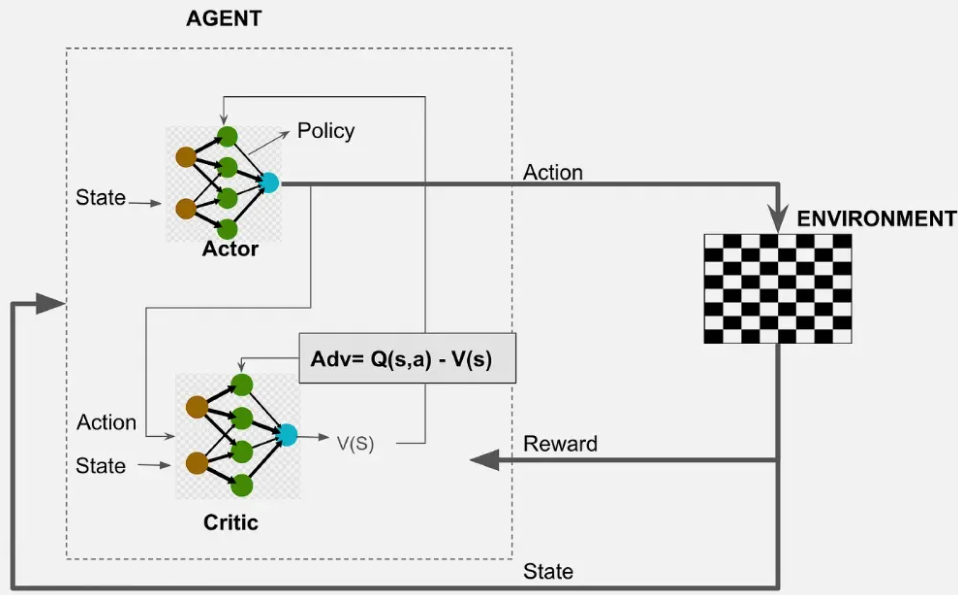
\includegraphics[width=0.75\linewidth]{a2c.png}
    \caption{Actor critic}
    \label{fig:placeholder}
\end{figure}
The \textbf{Actor-Critic} architecture provides a powerful and widely adopted method for solving RL problems, particularly in continuous action spaces. It employs two distinct neural networks:

\begin{itemize}
    \item \textbf{The Critic}: Learns a value function (typically the action-value function, $q_{\pi}(s, a)$). Its role involves evaluating actor decisions, providing supervisory signals in the form of Temporal Difference (TD) errors.
    
    \item \textbf{The Actor}: Represents the policy, $\pi(a|s)$. It receives current state inputs and outputs actions. It utilizes critic feedback—TD error—to update parameters via policy gradients, improving strategies over time.
\end{itemize}
\noindent
This architecture suits V2G applications well because it can directly learn policies over continuous action spaces, enabling fine-grained power control. Agent behavior is shaped entirely by received reward signals. Designing these signals to align agent objectives with desired multi-faceted goals represents a critical discipline known as reward engineering \cite{Xie2025, Zhang2023}.



% ===================================================================
% REWARD SHAPING SECTION
% ===================================================================
 \section{Reward Engineering: Shaping Agent Behavior}
\label{sec:reward_shaping}

The reward function is arguably the most critical component in a Reinforcement Learning system. It is the sole mechanism through which a designer can communicate the desired behavior to the agent. A poorly designed reward can lead to unintended and suboptimal behaviors, even if the agent successfully maximizes it. The entire field of reward engineering has become a cornerstone of modern RL, as it is fundamental to applying these algorithms effectively in complex, real-world applications \footcite{ibrahim2024comprehensive}. The V2G problem, with its multiple competing objectives—maximizing profit, ensuring user satisfaction, preserving battery health, and maintaining grid stability—makes reward design particularly challenging. This work explores several sophisticated techniques to guide the learning process effectively.

\subsection{Potential-Based Reward Shaping (PBRS)}
Potential-Based Reward Shaping (PBRS) is perhaps the most theoretically sound method for reward augmentation \footcite{ng1999policy}. It involves adding a shaping term, $F(s, s')$, to the environment's intrinsic reward, $R(s, a, s')$. The new, shaped reward $R'$ is thus defined as:
\[
R'(s, a, s') = R(s, a, s') + F(s, s')
\]
The shaping term itself is defined as the difference between a potential function, $\Phi$, evaluated at the new state and the old state:
\[
F(s, s') = \gamma \Phi(s') - \Phi(s)
\]
where $\gamma$ is the discount factor. The key theoretical guarantee of PBRS is \textbf{policy invariance}: adding a potential-based shaping reward does not change the optimal policy of the underlying MDP. While the agent learns the same optimal behavior, the shaping term can provide dense, intermediate rewards that significantly accelerate the learning process by guiding the agent's exploration.

\subsection{Dynamic and Adaptive Rewards}
Unlike PBRS, which provides a static reward bonus, a dynamic or adaptive reward function can evolve during training. This approach is particularly useful for complex problems where the relative importance of different objectives may change as the agent becomes more competent. For example, an agent could initially be rewarded simply for keeping an EV charged, but as training progresses, the reward function could adapt to introduce penalties for grid overloads or incentives for V2G services \footcite{wan2022dynamic}. This allows the agent to master different facets of the problem sequentially.

\subsection{Curriculum Learning}
While technically a training paradigm rather than a reward modification technique, Curriculum Learning (CL) is highly relevant to reward engineering. CL involves training the agent on a sequence of tasks that gradually increase in difficulty. In the V2G context, an agent might first be trained in a simple scenario with only a few EVs and stable prices. Once it masters this, it is moved to a more complex environment with more EVs, volatile prices, and hard constraints. This structured learning process prevents the agent from being overwhelmed by the full complexity of the problem from the start and can lead to more robust and generalizable policies.

\newpage
\section{The Rise of Deep Reinforcement Learning for V2G Control}

The convergence of RL with the substantial representational capabilities of deep neural networks has given rise to \textbf{Deep Reinforcement Learning (DRL)}, which currently represents the leading edge of V2G control research. The development of DRL algorithms has yielded a comprehensive toolkit, primarily divided into two main families: off-policy and on-policy methods, each exhibiting distinct operational characteristics.
The following figure illustrates the evolutionary relationships between the algorithms that  will be discussed, highlighting how newer ideas were built to overcome the limitations of their predecessors.

\begin{forest}
for tree={
grow=east,
parent anchor=east,
child anchor=west,
edge path={
\noexpand\path [draw] (!u.parent anchor) -- +(-0.5pt,0) |- (.child anchor)\forestoption{edge label};
},
draw,
rounded corners,
align=center,
l sep=7pt,
s sep=4pt,
minimum height=0.4cm,
inner sep=0.1pt,
anchor=west,
}
[RL Methods
[On-Policy
[Policy Gradient
[A2C]
[TRPO\\(Theoretical Stability)
[PPO\\(Practical Simplification)]
]
]
[Gradient-Free
[ARS\\(Random Search)]
]
]
[Off-Policy\\
[DDPG\\(Fundamental)
[DDPG+PER\\(Improve Sampling)]
[TD3\\(Resolve Overestimation)]
[SAC\\(Add Entropy)]
[TQC\\(Distributional Approach)]
]
]
]
\end{forest}
\subsection{Off-Policy Methods: Data-Efficient Learning from Experience}

Off-policy algorithms distinguish themselves through their capacity to learn optimal policies from data generated by different, often more exploratory, behavioral policies. This enables them to reuse historical experiences stored in large \textit{replay buffers}, breaking temporal correlation between experiences and achieving high sample efficiency.

\paragraph{Deep Deterministic Policy Gradient (DDPG)}

A foundational algorithm that successfully extended Deep Q-Networks (DQN) to high-dimensional, continuous action spaces, DDPG represented a significant breakthrough for control problems including V2G \footcite{lillicrap2015continuous}. It employs an actor-critic architecture where the actor deterministically maps states to actions. However, practical applications often encounter substantial training instability and systematic vulnerability to \textbf{overestimation bias}, where critic networks systematically overestimate Q-values, resulting in suboptimal policy learning \footcite{orfanoudakis2022deep, alfaverh2022optima}.

\paragraph{Twin Delayed DDPG (TD3)}

Developed as a direct successor to address DDPG's instabilities, TD3 introduces three key innovations that have become standard in contemporary DRL \footcite{fujimoto2018addressing}. It incorporates (1) clipped double Q-learning, utilizing paired critic networks and selecting minimum estimates to mitigate overestimation bias; (2) delayed policy updates, updating actors less frequently than critics for enhanced stability; and (3) target policy smoothing, adding noise to target actions for learning regularization. These enhancements establish TD3 as a more robust and reliable baseline for complex V2G applications \footcite{liu2023optimal, wang2022multi}.

\paragraph{Soft Actor-Critic (SAC)}

SAC represents a state-of-the-art off-policy algorithm for continuous control, recognized for superior sample efficiency and stability \footcite{haarnoja2019soft}. Its fundamental innovation involves the \textbf{maximum entropy framework}. The agent's objective is modified to maximize both expected reward and policy entropy. This entropy bonus encourages agents to act as randomly as possible while maintaining task success, promoting broader exploration, improved noise robustness, and reduced risk of poor local optima convergence \footcite{logeshwaran2022comparative}.

\paragraph{Truncated Quantile Critics (TQC)}

TQC addresses overestimation bias through a distributional RL approach \footcite{kuznetsov2020controlling}. Rather than learning single expected returns (Q-values), its critic learns complete return probability distributions using quantile regression. By learning multiple return distribution quantiles and truncating the most optimistic quantile estimates before averaging, it provides a more principled and effective method for removing primary overestimation bias sources, frequently achieving superior performance.

\paragraph{Enhancement: Prioritized Experience Replay (PER)}

This represents not a standalone algorithm but a crucial orthogonal modification for off-policy methods. Standard replay buffers sample past transitions uniformly. PER samples transitions based on their "importance," typically proportional to TD error magnitude \footcite{schaul2015prioritized}. This focuses learning processes on surprising or informative experiences, significantly accelerating convergence and improving final performance.

\subsection{On-Policy Methods: Stability through Cautious Updates}

On-policy methods learn exclusively from data generated by current policies being optimized. Once data is used for updates, it is discarded. While this makes them inherently less sample-efficient than off-policy counterparts, their updates often demonstrate greater stability and reduced divergence risk.

\paragraph{Advantage Actor-Critic (A2C/A3C)}

A2C represents a foundational synchronous, on-policy Actor-Critic algorithm. Its powerful extension, \textbf{Asynchronous Advantage Actor-Critic (A3C)}, was a landmark contribution demonstrating parallelism benefits \footcite{mnih2016asynchronous}. A3C utilizes multiple parallel workers, each with individual model and environment copies. These workers interact with their environments independently, and collected gradients update a global model asynchronously. This decorrelates data streams and provides powerful stabilizing effects on learning processes.

\paragraph{Trust Region Policy Optimization (TRPO)}

TRPO was the first algorithm to formalize policy update size constraints for guaranteed monotonic policy improvement \footcite{schulman2020trust}. It maximizes a "surrogate" objective function subject to policy change constraints, measured by Kullback-Leibler (KL) divergence. This creates a "trust region" within which new policies are guaranteed to improve upon previous ones, preventing catastrophic updates that can permanently derail learning. However, implementation complexity arises from second-order optimization requirements.

\paragraph{Proximal Policy Optimization (PPO)}

PPO achieves TRPO's stability benefits and reliable performance using only first-order optimization, making it far simpler to implement and more broadly applicable \footcite{schulman2017proximal}. It employs a novel \textbf{clipping} mechanism in its objective function to discourage large policy updates that would move new policies too far from previous ones, effectively creating "soft" trust regions. Due to its excellent balance of performance, stability, and implementation simplicity, PPO has become a default choice for many on-policy applications.

\subsection{Gradient-Free Methods: An Alternative Path}

\paragraph{Augmented Random Search (ARS)}

As a counterpoint to dominant gradient-based methods, ARS represents a gradient-free approach that optimizes policies directly in parameter space \footcite{mania2018simple}. It operates by exploring random policy parameter perturbations and updating central policy parameter vectors based on observed performance of these perturbations. While often less sample-efficient for complex, high-dimensional problems, its extreme simplicity, scalability, and robustness to noisy rewards can make it competitive in certain domains.

\section{The Model-Based Benchmark: Model Predictive Control (MPC)}

While DRL offers powerful model-free approaches, academic rigor requires benchmarking against its most robust model-based counterpart: \textbf{Model Predictive Control (MPC)}. MPC originated in the 1970s within the process control industry, with pioneering contributions by Richalet et al. \footcite{Richalet1978ModelPH} and Cutler and Ramaker \footcite{Cutler1980}. The theoretical foundations for stability and optimality were subsequently established rigorously by researchers including Mayne and Rawlings \footcite{mayne2000constraine}.
\noindent
At its core, MPC represents a proactive, forward-looking strategy that employs explicit mathematical system models to predict future evolution. At each control step, it solves finite-horizon optimal control problems to determine optimal control action sequences. Its primary strength, explaining widespread industrial adoption, lies in its inherent capability to proactively handle complex system dynamics and operational constraints \footcite{minchala2025systematic}.

\subsection{Implicit MPC: Online Optimization}

The most common formulation involves \textbf{Implicit MPC}, where constrained optimization problems are solved online at each control step. For linear systems with quadratic costs, this typically constitutes a Quadratic Programme (QP). The controller's objective involves finding future control input sequences $U = [u_{t|t}, ..., u_{t+N-1|t}]$ that minimize cost function $J$ over prediction horizon $N$.

\begin{equation}
\min_{U} J(x_t, U) = \sum_{k=0}^{N-1} (x_{t+k|t}^T Q x_{t+k|t} + u_{t+k|t}^T R u_{t+k|t}) + x_{t+N|t}^T P x_{t+N|t}
\end{equation}
\noindent
where $x_{t+k|t}$ represents predicted state at future step $k$ based on time $t$ information, and $Q$, $R$, and $P$ are weighting matrices defining trade-offs between state deviation and control effort. This optimization is subject to system dynamics models and operational constraints:

\begin{gather}
    x_{t+k+1|t} = A x_{t+k|t} + B u_{t+k|t} \\
    x_{min} \le x_{t+k|t} \le x_{max} \\
    u_{min} \le u_{t+k|t} \le u_{max}
\end{gather}
\noindent
At each time step $t$, this complete problem is solved, but only the first action of the optimal sequence, $u_{t|t}^*$, is applied to the system. The process then repeats at the next time step, $t+1$, using new system state measurements. This feedback mechanism, known as a \textit{receding horizon} strategy, makes MPC robust to disturbances and model mismatch.

\cite{camacho2013model} \cite{borrelli2017predictive}

\subsection{Explicit MPC: Offline Pre-computation}

For systems with fast dynamics or limited online computational capacity, \textbf{Explicit MPC} offers an alternative approach. Here, constrained optimization problems are solved offline for all possible initial states within given ranges, using multi-parametric programming. The result is not an online algorithm, but a pre-computed, explicit control law, $\pi(x_t)$, which is a \textbf{piecewise affine function} of state vector $x_t$.

\begin{equation}
u^*(x_t) = F_i x_t + g_i \quad \text{if } x_t \in \mathcal{X}_i
\end{equation}
\noindent
The state space is partitioned into convex polyhedral region sets $\mathcal{X}_i$, with unique affine control laws defined for each region. Online operation then reduces to fast lookup operations to identify which region current state $x_t$ occupies and applying the corresponding simple control law. This trades very high offline computational burden and significant memory requirements for extremely fast online execution.

\cite{bemporad2013explicit} \cite{borrelli2017predictive}



\section{A Comparative Perspective on Control Methodologies}

While DRL represents the cutting edge, contextualizing it within the broader control strategy landscape remains crucial for academic rigor. The choice between learning-based, model-free approaches and optimization-based, model-based approaches represents fundamental philosophical and practical trade-offs.

\begin{table}[H]
\centering
\caption{Comparative Analysis: DRL vs. Model Predictive Control (MPC) for V2G}
\label{tab:drl_vs_mpc}
\resizebox{0.8\textwidth}{!}{
\begin{tabular}{|p{0.2\linewidth}|p{0.35\linewidth}|p{0.35\linewidth}|}
\hline
\textbf{Aspect} & \textbf{Deep Reinforcement Learning (DRL)} & \textbf{Model Predictive Control (MPC)} \\
\hline
\textbf{Paradigm} & Model-Free, learning-based. Learns an optimal policy (a reactive function) via trial-and-error interaction with the environment. & Model-Based, optimisation-based. Solves a constrained optimisation problem at each time step based on a system model and forecasts. \\
\hline
\textbf{Strengths} & \begin{itemize} \item Highly robust to uncertainty and unmodelled stochasticity. \item Does not require an explicit, accurate system model. \item Can learn complex, non-linear control policies. \item Extremely fast inference time (a single forward pass) once trained. \end{itemize} & \begin{itemize} \item Explicitly and rigorously handles hard constraints, providing safety guarantees. \item Proactive and anticipatory if forecasts are accurate. \item Well-established, mature, and theoretically understood. \end{itemize} \\
\hline
\textbf{Weaknesses} & \begin{itemize} \item Can be highly sample-inefficient during the training phase. \item Lacks hard safety guarantees (an active and important area of research). \item The "black box" nature of neural network policies can make them difficult to interpret or verify. \end{itemize} & \begin{itemize} \item Performance is fundamentally shackled to the accuracy of the system model and external forecasts. \item Computationally expensive at each time step, suffering from the "curse of dimensionality" with system size. \item Can be brittle to unexpected forecast errors and unmodelled dynamics. \end{itemize} \\
\hline
\textbf{V2G Suitability} & Excellent for dynamic, highly uncertain environments with complex, non-linear trade-offs and a large number of assets. & Good for problems with simple, well-defined dynamics and reliable forecasts, but struggles with the real-world stochasticity and scale of V2G. \\
\hline
\end{tabular}
}
\end{table}

\noindent
\textbf{Model Predictive Control (MPC)} stands as the most powerful model-based alternative \footcite{alsabbagh2022reinforcement}. Its primary and most compelling strength lies in its native ability to handle hard constraints, which is critical for ensuring safe operation (such as never violating transformer limits or user energy requirements). However, its performance remains fundamentally constrained by the accuracy of its internal model and forecasts of future disturbances (prices, user behavior) \footcite{faggio2023design}. In practice, creating accurate, tractable models for the entire V2G domain proves nearly impossible due to non-linear battery dynamics, extreme market volatility, and the profound unpredictability of human behavior. Furthermore, as EV fleet sizes grow, optimization problem dimensionality explodes, making online computation required at each time step intractable for large fleets \footcite{schwenk2022computationally}.

\noindent
Other methods, such as \textbf{meta-heuristic algorithms} (including genetic algorithms and particle swarm optimization), are sometimes proposed. However, these are typically employed for offline scheduling and lack the real-time, reactive responsiveness required for dynamic V2G control in rapidly changing environments \footcite{kumar2024integration}.

\noindent
Ultimately, DRL's singular advantage lies in its ability to learn and internalize the complex, non-linear trade-offs of multi-objective V2G problems directly from data, without requiring explicit models. This makes it uniquely suited to navigating the profound uncertainties of real-world operations. While other methods have their applications, DRL stands out as the most promising technology for deploying truly intelligent, autonomous, and scalable V2G management systems required to achieve the ambitious energy and climate objectives of the European Union.

\newpage
\section{A Primer on Lithium-Ion Battery Chemistries and Degradation}

The effectiveness, safety, and economic viability of any V2G strategy remain fundamentally constrained by the physical and chemical characteristics of vehicle batteries. Battery chemistry selection dictates EV operational envelopes, influencing energy density, power capabilities, lifespan, and safety profiles. Clear understanding of these trade-offs proves essential for developing robust, realistic, and responsible control algorithms.

\subsection{Fundamental Concepts and Degradation Mechanisms}

Battery degradation represents a complex, irreversible process that reduces battery capacity to store and deliver energy. It manifests primarily as capacity reduction (energy fade) and internal resistance increases (power fade). The mechanisms are broadly categorized into two types: calendar aging and cyclic aging \footcite{birkl2017degradation}.

\begin{itemize}
    \item \textbf{Calendar Aging:} This refers to degradation occurring while batteries remain at rest, whether fully charged or empty. The primary, unavoidable mechanism involves slow, continuous growth of the \textbf{Solid Electrolyte Interphase (SEI)} layer on graphite anode surfaces. While thin, stable SEI layers are necessary for battery function, continued growth represents a parasitic reaction consuming active lithium ions and electrolyte, leading to irreversible capacity loss. SEI growth rates are strongly accelerated by two main factors:
    \begin{itemize}
        \item \textbf{High Temperature:} Higher temperatures increase all chemical reaction rates, including parasitic ones. Storing batteries in hot environments proves highly detrimental.
        \item \textbf{High State of Charge (SoC):} High SoC corresponds to low electrochemical potential at the anode, making graphite more reactive with electrolyte, thus promoting faster SEI growth \footcite{vetter2005ageing}. This explains why leaving EVs stored at 100\% SoC for extended periods is discouraged.
    \end{itemize}

    \item \textbf{Cyclic Aging:} This refers to degradation occurring as a direct result of charging and discharging batteries. V2G operations directly contribute to this aging type. Key mechanisms include:
    \begin{itemize}
        \item \textbf{Mechanical Stress:} During charging and discharging, lithium ions intercalate and de-intercalate from electrode materials, causing expansion and contraction. This repeated mechanical stress can cause micro-cracks in electrode particles, leading to electrical contact loss and active material reduction, thereby causing capacity fade. This effect becomes more pronounced with larger \textbf{Depths of Discharge (DoD)}.
        \item \textbf{SEI Layer Instability:} Volume changes from cycling can also crack protective SEI layers, exposing fresh anode material to electrolyte and triggering further, accelerated SEI growth.
        \item \textbf{Lithium Plating:} This represents a particularly damaging mechanism occurring under stressful conditions, such as very high charging rates (high C-rates) or low temperatures. Instead of smoothly intercalating into graphite anodes, lithium ions deposit on anode surfaces as metallic lithium. This causes rapid and severe capacity loss and can form sharp, needle-like structures called dendrites, which pose severe safety risks as they can grow through separators and cause internal short circuits \footcite{birkl2017degradation}.
    \end{itemize}
\end{itemize}
\noindent
For V2G applications, which inherently involve frequent and potentially deep cycling, understanding and mitigating cyclic aging remains paramount for ensuring long-term technology viability.

\subsection{Key Automotive Chemistries}

The EV market is dominated by several key lithium-ion battery families, primarily distinguished by cathode materials. Each chemistry presents different balances of performance characteristics.

\begin{itemize}
    \item \textbf{Lithium Nickel Manganese Cobalt Oxide (NMC):} For years, this has been the most popular choice due to its excellent balance of energy density, power, and cycle life. The ratio of Nickel, Manganese, and Cobalt can be adjusted (such as NMC111, NMC532, NMC811) to prioritize either energy density (high Nickel) or safety and longevity (lower Nickel).
    
    \item \textbf{Lithium Nickel Cobalt Aluminum Oxide (NCA):} Offers very high specific energy (energy density by weight), enabling longer vehicle range. However, it typically comes at the cost of slightly lower cycle life and narrower safety margins compared to NMC, requiring more sophisticated thermal management.
    
    \item \textbf{Lithium Iron Phosphate (LFP):} Is rapidly gaining market share, particularly in standard-range vehicles, due to lower cost (no cobalt, an expensive and ethically contentious material) and superior safety. LFP batteries offer exceptional cycle life (often 3-4 times that of NMC/NCA) and are considered the safest common Li-ion chemistry due to high thermal stability. Their main drawback involves lower energy density.
    
    \item \textbf{Lithium Titanate Oxide (LTO):} This represents a more niche chemistry using titanate-based anodes instead of graphite. This provides exceptional safety (virtually no thermal runaway risk), extremely long cycle life (>10,000 cycles), and excellent low-temperature performance. However, very low energy density and high cost currently limit its use to specialized applications.
\end{itemize}

\subsection{Voltage Profiles and the Challenge of SoC Estimation}

The relationship between battery open-circuit voltage and SoC represents a critical, non-linear function unique to each chemistry. The derivative of cell voltage with respect to DoD, $\frac{dV_{cell}}{d(DoD)}$, constitutes a key parameter for Battery Management Systems (BMS). Steep, monotonic slopes allow BMS to accurately infer SoC from simple voltage measurements. Conversely, flat slopes make this estimation extremely difficult.

\begin{figure}[H]
    \centering
    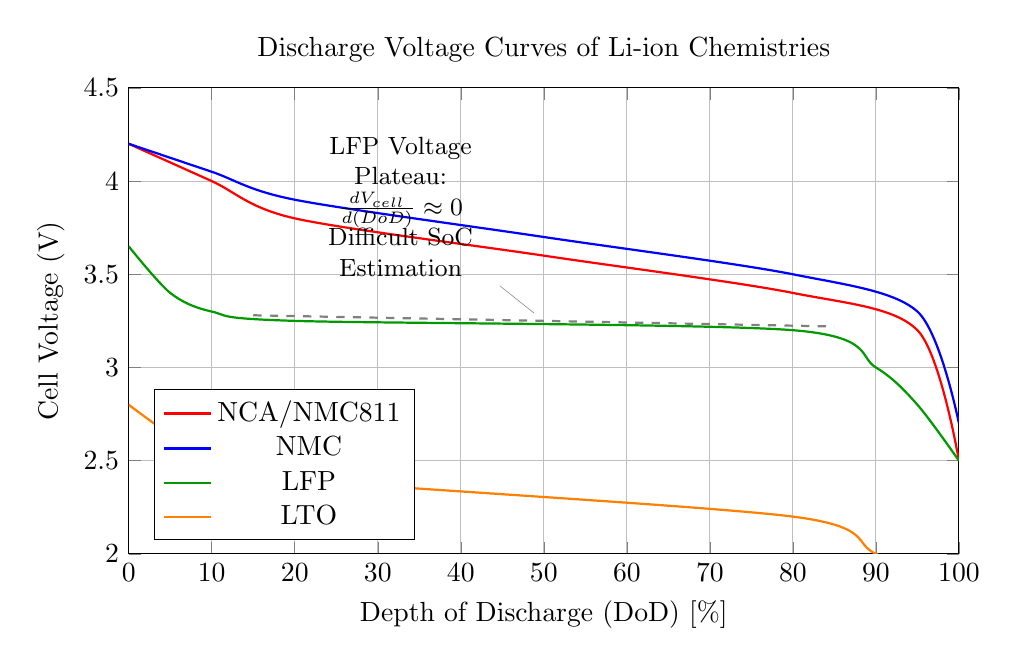
\begin{tikzpicture}
        \begin{axis}[
            title={Discharge Voltage Curves of Li-ion Chemistries},
            xlabel={Depth of Discharge (DoD) [\%]},
            ylabel={Cell Voltage (V)},
            xmin=0, xmax=100,
            ymin=2.0, ymax=4.5,
            grid=major,
            legend pos=south west,
            width=\textwidth,
            height=7.5cm,
        ]
        \addplot[smooth, thick, red] coordinates { (0, 4.2) (10, 4.0) (20, 3.8) (50, 3.6) (80, 3.4) (95, 3.2) (100, 2.5) };
        \addlegendentry{NCA/NMC811}

        \addplot[smooth, thick, blue] coordinates { (0, 4.2) (10, 4.05) (20, 3.9) (50, 3.7) (80, 3.5) (95, 3.3) (100, 2.7) };
        \addlegendentry{NMC}

        \addplot[smooth, thick, green!60!black] coordinates { (0, 3.65) (5, 3.4) (10, 3.3) (20, 3.25) (80, 3.2) (90, 3.0) (95, 2.8) (100, 2.5) };
        \addlegendentry{LFP}
        
        \addplot[smooth, thick, orange] coordinates { (0, 2.8) (10, 2.5) (20, 2.4) (80, 2.2) (90, 2.0) (100, 1.8) };
        \addlegendentry{LTO}

        \draw[dashed, thick, gray] (axis cs:15,3.28) -- (axis cs:85,3.22);
        \node[pin=135:{\parbox{2.5cm}{\centering \small LFP Voltage Plateau: \\ $\frac{dV_{cell}}{d(DoD)} \approx 0$ \\ Difficult SoC Estimation}}] at (axis cs:50,3.25) {};
        \end{axis}
    \end{tikzpicture}
    \caption{Typical discharge voltage curves for various lithium-ion chemistries. The extremely flat profile of LFP makes accurate SoC estimation challenging based on voltage alone, necessitating more complex estimation techniques like Coulomb counting and periodic recalibration\footcite{plett2015battery}.}
    \label{fig:voltage_curves_detailed}
\end{figure}
\noindent
As shown in Figure \ref{fig:voltage_curves_detailed}, LFP's remarkably flat voltage plateau makes it nearly impossible for BMS to determine precise SoC in the central operating range (from approximately 20\% to 80\%) using voltage alone. This necessitates more complex estimation techniques, such as Coulomb counting (integrating current over time), which can suffer from drift. To correct this drift, LFP-equipped vehicles require periodic full charges to 100\% for BMS recalibration. This represents an important operational constraint that V2G control strategies must consider.

\subsection{Comparative Analysis and Safety Considerations}

The trade-offs between chemistries are summarized in Table \ref{tab:chem_comparison_detailed}. Safety remains paramount, with the primary risk being thermal runaway—a dangerous, self-sustaining exothermic reaction. This risk relates directly to cathode material chemical and thermal stability. Higher energy density generally means more energy packed into smaller mass, which can be released violently if cells are compromised. Consequently, critical temperatures for initiating thermal runaway are generally lower for higher energy density chemistries. LFP's stable phosphate-based structure makes it far more resistant to thermal runaway than nickel-based counterparts, a key reason for its growing popularity.

\begin{table}[h!]
\centering
\small
\caption{Comparative analysis of key automotive battery chemistries, highlighting the trade-offs between performance and safety.}
\label{tab:chem_comparison_detailed}
\begin{tabularx}{\textwidth}{
  @{}
  >{\bfseries\RaggedRight}X
  *{5}{C}
  @{}
}
\toprule
Metric & NCA & NMC & LFP & LTO & LCO \\
\midrule
Energy Density (Wh/kg) & 200 - 260 (Highest) & 150 - 220 (High) & 90 - 160 (Moderate) & 60 - 110 (Low) & 150-200 (High) \\
\addlinespace
Cycle Life & 1000 - 2000 & 1000 - 2500 & 2000 - 5000+ & $>$10,000 & 500 - 1000 \\
\addlinespace
Safety & Good & Very Good & Excellent & Excellent & Poor \\
\addlinespace
Thermal Runaway Temp ($^{\circ}$C) & $\sim$150 - 180 & $\sim$180 - 210 & $\sim$220 - 270 & $>$ 250 & $\sim$150 \\
\bottomrule
\end{tabularx}
\end{table}